\chapter{Method} \label{sec:method}
\section{Design Philosophy}
\subsection{Use of Pure Functions}
One of the most notable differences of the \moozi implementation compared to other implementations is the use of pure functions.
In \moozi, we separate the storage of data and the handling of data whenever possible, especially for the parts with heavy computations.
We use \textbf{JAX} and \textbf{Haiku} \cite{HaikuSonnetJAX_Hennigan.Cai.ea_2020,JAXComposableTransformations_JamesBradbury.RoyFrostig.ea_2018} to implement neural network related modules (see Section \ref{sec:jax_and_podracer}).
These libraries separate the \textbf{specification} and the \textbf{parameters} of a neural network.
The \textbf{specification} of a neural network is a pure function that is internally represented by a fixed computation graph.
The \textbf{parameters} of a neural network includes all learned network weights that can be used with the specification to perform a forward pass.
For example, given a simple neural network with a single dense layer that computes
\begin{align*}
    \mathbf{y} = \operatorname{tanh}\left( \mathbf{A}\mathbf{x} + \mathbf{b} \right)
\end{align*}
Here $\mathbf{x}$ is the input vector of shape $(n, 1)$, $\mathbf{y}$ is the output vector of shape $(m, 1)$, $\mathbf{A}$ are the learned weights of shape $(m, n)$, and $b$ is the learned bias of shape $(m, 1)$.
The parameters are all the weights in $\mathbf{A}$ and $b$.
We demonstrate how to build this simple network using JAX and Haiku in Algorithm \ref{code:pure}.
We visualize the computation graph of it in Figure \ref{fig:pure}.
\includecode{pure}{
    \textbf{A simple dense layer implemented in JAX and Haiku.}
    The \textit{model} in the code is the specification of the neural network.
    The \textit{params} in the code is the parameters of the neural network.
    Only \textit{params} contains concrete data.
}
\includeimage[0.4]{pure}{
    \textbf{Computation graph of the simple dense layer in Algorithm \ref{code:pure}.}
}{
    This computation graph show no concrete data, but the data types, shapes, and operators of the layer (\textit{f32} stands for \textit{single-precision float}).
    To complete a forward pass, we need both concrete neural network parameters \textit{args[0]} ($\mathbf{A}, \mathbf{b}$) and a concrete input value \textit{args[1]} ($\mathbf{x}$).
}
Using these pure functions separates the \textit{algorithm} of the agent and the \textit{state} of the agent both conceptually and in implementation.
The \textit{algorithm} part of the agent can be abstracted into a computation graph that can be compiled and optimized using a specialized compiler, such as XLA \cite{TensorFlowLargescaleMachine_Abadi.Agarwal.ea_2015}, for hardware acceleration (see Section \ref{sec:jax_and_podracer}).
The \textit{state} part of the agent can be efficiently handled by tools specialized in data manipulations and transferring such as Ray (see Section \ref{sec:ray}).
This way, our system efficiently performs inferences on accelerators (such as GPUs and TPUs) and transfers data on CPUs.
% \note{I think this section is too verbose. I should probably cut it to half a page.}

\subsection{Training Efficiency}
In Section \ref{sec:drl_systems} we reviewed common DRL systems for which their developers stated training efficiency as the highest priority in their system design.
We also designed our system efficient and scalable.
Here we describe key features of our system which improve its efficiency.
The first one is system parallelization.
The computation throughput of a single process is simply not enough for DRL systems.
In the published results of MuZero by \cite{MasteringAtariGo_Schrittwieser.Antonoglou.ea_2020}, the agent generated over 20 billion environment frames for training.
For a non parallelized system, consider Gymnax's efficient \textit{MinAtar} implementation where each environment step takes about 1 millisecond \cite{GymnaxJAXbasedReinforcement_RobertTjarkoLange_2022}.
A single process would take more than 200 days just to step the environment, without considering the model training cost.
As a result, we have to build a distributed system to increase total throughput through parallelism.

The second key feature of our system is the environment transition speed.
In Atari games, especially Atari games in ALE (\ref{sec:ale}), taking one environment step invokes a full-fledged Atari emulator in the backend, which is much more time consuming than neural network inference.
Board games, especially those are implemented in high performance languages, are much faster.
We use \textit{MinAtar} (reviewed in Section \ref{sec:min_atar}) for simpler variants of Atari games, and \textit{OpenSpiel} for efficient implementations of board games to reduce the time spent on environment transitions \cite{OpenSpielFrameworkReinforcement_Lanctot.Lockhart.ea_2020,MinAtarAtariInspiredTestbed_Young.Tian_2019}.

The third key feature is efficient acting with interdependent inferences.
DRL systems such as IMPALA assume that the policy output can be computed by a single forward pass of a neural network.
However, MuZero's policy requires multiple inferences per action taken and these inferences are dependent on each other based on the tree search.
Our system, utilizing JAX and MCTX, handles acting with multiple inferences per action efficiently by implementing the entire process of acting in native JAX.

\subsection{Understanding the Method is Important}
Machine learning algorithms, especially those involving neural networks, have interpretability issues and sometimes can only be used as ``black boxes'' \cite{ExplainableAIReview_Linardatos.Papastefanopoulos.ea_2021}.
We believe that having a system that we can understand is much more useful for future research than having a system that ``just works''.
Therefore, our project studies the behavior of the system through extensive logging and visualization utilities.
% We will show we use these tools to understand the learned model in section \ref{sec:logging}.

\section{Architecture Overview}
In \moozi, we use the \textbf{Ray} library designed by \citeauthor{RayDistributedFramework_Moritz.Nishihara.ea_2018} \cite{RayDistributedFramework_Moritz.Nishihara.ea_2018} for orchestrating distributed processes.
We also adopt the terminology used by Ray.
In a distributed system with \textbf{centralized control}, a single \textbf{driver} process is responsible for operating all other processes.
Other processes are either \textbf{tasks} or \textbf{actors}.
\textbf{Tasks} are stateless functions that take inputs and return outputs.
\textbf{Actors} are stateful objects that can perform multiple tasks.
In the RL literature, \textbf{actor} is also a commonly used term for describing the process that holds a copy of the network weights and interacts with an environment \cite{SEEDRLScalable_Espeholt.Marinier.ea_2020, IMPALAScalableDistributed_Espeholt.Soyer.ea_2018}.
Even though \moozi does not adopt this concept of a RL actor, we will use the terms \textbf{Ray task} and \textbf{Ray actor} to avoid confusion.
In contrast to distributed systems with \textbf{distributed control}, ray tasks and actors are reactive and do not have busy loops.
The driver controls when a ray task or actor is activated, what data is used as input, and where the output go.
The driver orchestrates the data and control flow of the entire system.
Ray tasks and actors merely respond to instructions, process input and return output on command.
We illustrate \moozi's architecture in Figure \ref{fig:moozi_architecture}.
\note{I recently simplied the names of the workers. I will update this graph later.}

\begin{figure}[htbp]
    \captionsetup{width=\textwidth}
    \centering
    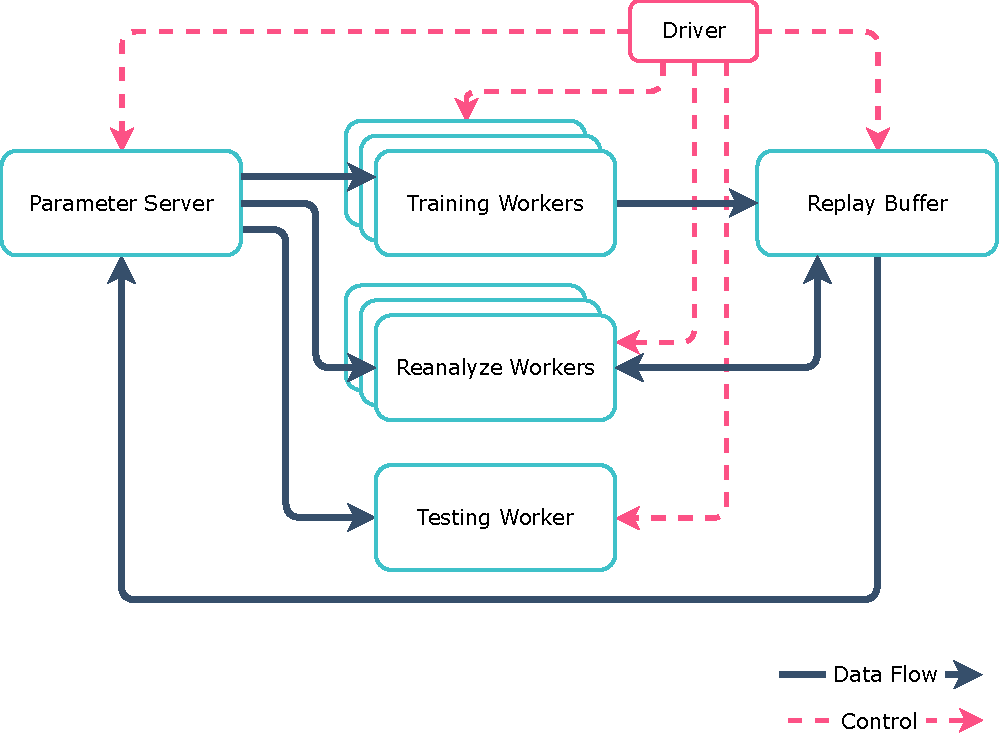
\includegraphics[width=0.8\textwidth, height=0.8\textheight,keepaspectratio]{assets/moozi_architecture.pdf}
    \caption[\textbf{The \moozi Architecture.}]{
        \textbf{The \moozi Architecture.}
        The \textit{Driver} is the entry point of the program (\ref{sec:driver}).
        The \textit{Parameter Server} stores the latest copy of the network weights and performs batched updates to them (see Section \ref{sec:param_server}).
        The \textit{Replay Buffer} stores generated trajectories and processes these trajectories into training targets (see Section \ref{sec:replay}).
        A \textit{Training Worker} is a ray actor responsible for generating experiences by interacting with the environment (see Section \ref{sec:train_rw}).
        A \textit{Testing Worker} is a ray actor responsible for evaluating the system by interacting with the environment (see Section \ref{sec:test_rw}).
        A \textit{Reanalyze Worker} is a ray actor that updates search statistics for history trajectories (see Section \ref{sec:re_w}).
    }
    \label{fig:moozi_architecture}
\end{figure}

% \includeimage[0.8]{moozi_architecture}{
%     \textbf{The \moozi Architecture.}
% }{
%     The \textit{Driver} is the entry point of the program (\ref{sec:driver}).
%     The \textit{Parameter Server} stores the latest copy of the network weights and performs batched updates to them (see Section \ref{sec:param_server}).
%     The \textit{Replay Buffer} stores generated trajectories and processes these trajectories into training targets (see Section \ref{sec:replay}).
%     A \textit{Training Worker} is a ray actor responsible for generating experiences by interacting with the environment (see Section \ref{sec:train_rw}).
%     A \textit{Testing Worker} is a ray actor responsible for evaluating the system by interacting with the environment (see Section \ref{sec:test_rw}).
%     A \textit{Reanalyze Worker} is a ray actor that updates search statistics for history trajectories (see Section \ref{sec:re_w}).
% }

\section{The \moozi System Components}
\subsection{Environment Bridges} \label{sec:env_bridge}
Environment bridges unify environments which are defined in different libraries to a shared interface used by \moozi.
In software engineering terms, environment bridges follow the \textbf{bridge design pattern} \cite{BridgePattern__2022}.
In our project we implement environment bridges for three types of environments that are commonly used in RL research: \textit{OpenAI Gym}, \textit{OpenSpiel}, and \textit{MinAtar} \cite{OpenAIGym_Brockman.Cheung.ea_2016,OpenSpielFrameworkReinforcement_Lanctot.Lockhart.ea_2020,MinAtarAtariInspiredTestbed_Young.Tian_2019}.
% The bridges wrap these environments into the \textbf{The DeepMind RL Environment API} \cite{DmEnvDeepMind__2022}.
% In this format, each environment step outputs a four-tuple (\textit{step type}, $r$, $\gamma$, $o$), where $r, \gamma, o$ are reward, discount, and partial observation respectively.
% The \textit{step type} is an enumerated value which indicates the type of timestep.
% The three possible values of \textit{step type} are (1) \textit{first}, indicating the start of an episode,
% (2) \textit{mid}, indicating an intermediate step, and (3) \textit{last} indicating the last step of an episode.

For all these wrapped environments, our bridges produce a flat structure for each timestep that has the following:
\begin{itemize}
    \item Inputs
          \subitem $b^{\text{last}}_{t}$: A boolean indicating the episode end.
          \subitem $a_t$: An integer encoding of the action taken.
    \item Outputs
          \subitem $o_t$:
          An N-dimensional array representing the observation of the current timestep as an image
          in the shape $(H, W, C_e)$. $H$ is the height, $W$ is the width, and $C_e$ is the number of channels.
          \subitem $b^{\text{first}}_{t}$: A boolean indicating the episode start.
          \subitem $b^{\text{last}}_{t}$: A boolean indicating the episode end.
          \subitem $b^{\text{player}_{t}}$: A boolean indicating the current player. A boolean is sufficient because \moozi currently only supports environments with at most two players.
          \subitem $r_t$: A float indicating the reward of taking the given action.
          \subitem $m^{A^a}_t$: A bit mask indicating legal action indices. Valid
          action indices are $1$ and invalid actions indices are $0$ for non-terminal states (see Section \ref{sec:a_aug}).
          %   \note{remove this as it's not use}
\end{itemize}

All environments are generalized to continuous tasks by passing an additional input $b^\text{last}_t$ to the environment stepping argument.
For an episodic task, the environment is reset internally when $b^{\text{last}}_t$ is \textit{True}.
The policy still executes for the last environment step, but the resulting action is discarded.
For a continuous task, the environment always steps with the latest action and never sets $b^\text{last}$ to \textit{true}.
Algorithm \ref{code:env_interface} demonstrates the unified main loop interface.
\includecode{env_interface}{
    \textbf{Unified Main Loop Interface.}
    Both \textit{episodic} environments and \textit{continuous} environments are handled with the same main loop.
}
We also implement a mock environment \cite{MockObject__2021} using the same interface.
A mock environment is initialized with a \textbf{trajectory sample} $\mathcal{T}$, and simulates the environment by outputting step samples one at a time.
An agent can interact with this mock environment as if it were a real environment.
However, the actions taken by the agent do not affect the state transitions since they are predetermined by the given trajectory from initialization.
This mock environment is used by the reanalyze workers in Section \ref{sec:re_w}.


\subsection{Vectorized Environment} \label{sec:vec_env}
A vectorized environment supervisor stacks multiple individual environments to form a single vectorized environment.
The environment takes inputs and produces outputs similar to an individual environment, but with an additional batch dimension.
For example, an individual environment produces a single frame of shape $(H, W, C)$, while the vectorized environment produces a batched frame of shape $(B, H, W, C)$.
Previously scalar outputs such as reward are also stacked into vectors of size $B$.
Since environment bridges generalize episodic tasks as continuous tasks, we do not need special handling for the first and the last timesteps in the vectorized environment and its main loop looks exactly like that in Algorithm \ref{code:env_interface}.
Using vectorized environments increases the communication bandwidth between the environment and the agent and facilitates designing a vectorized agent that processes batched inputs and returns batched actions in one call.

The mock environment described in Section \ref{sec:env_bridge} is less trivial to vectorize.
Each mock environment has to be initialized with a trajectory sample.
To vectorize $B$ mock environments, at least $B$ trajectories have to be tracked at the same time.
These $B$ trajectories usually have different length and therefore terminate at different timesteps.
Once one of the mocked trajectories reaches its termination, another trajectory has to fill the slot.
We create a trajectory buffer to address this problem.
When a new trajectory is needed by one of the mocked environments, the buffer replenishes it,
so the vectorized mocked environment can process batched interactions like a regular vectorized environment until the trajectory buffer runs out of trajectories.
An external process has to refill the buffer once in a while.
The driver pulls the latest trajectories from the replay buffer and supplies the mock environment's trajectory buffer (also see Section \ref{sec:re_w}).

\subsection{Action Space Augmentation} \label{sec:a_aug}
We augment the action space by adding a dummy action $a^\text{dummy}$ indexed at 0.
This dummy action is used to construct history observations when the horizon extends beyond the current timestep.
For example, if the history horizon is 3, we need the last three frames and actions to construct the input observation to the policy.
However, if the current timestep is 0, the agent hasn't taken any actions yet.
We use zeroed frames with the same shape as history frames, and the dummy action as history actions.
Moreover, \moozi's planner (see Section \ref{sec:planner}) does not have access to a perfect model, and it does not know when a node represents a terminal state.
Node expansions do not stop at terminal states and the tree search can simulate multiple steps beyond the end.
Search performed in these invalid subtrees not only wastes precious search budget, but also back-propagates value and reward estimates that are not learned from generated experience.
We address this issue by letting the model learn a policy that always takes the dummy action beyond a terminal state.
This learned dummy action acts as a switch that, once taken, treats all nodes in its subtree as absorbing states and edges that have zero value and reward respectively.
This discourages the planner from searching in invalid regions and improves search performance for near-end game states.
To formally differentiate these two types of action spaces, we denote the original environment action space $\mathcal{A}^e$ and the augmented action space $\mathcal{A}^a$, with
\begin{align*}
    \mathcal{A}^a  & = \mathcal{A}^e \cup \lbrace a^\text{dummy} \rbrace  \\
    a_{i}          & = a^\text{dummy} ~~~~ \forall i < 0                  & \text{(before the first timestep)}  \\
    a_{i}          & = a^\text{dummy} ~~~~ \forall i \geq T               & \text{(after the last timestep)}  \\
\end{align*}
Notice that the environment terminates at timestep $T$ so the last effective action taken by the agent is $a_{T-1}$.

\subsection{History Stacking} \label{sec:history_stacking}
In fully observable environments, the state $s_t$ at timestep $t$ observed by the agent entails sufficient information about the future state distribution.
However, for partially observable environments, this does not hold.
The optimal policy might not be representable by a policy $\pi(a \mid o_t)$ that only takes into account the most recent partial observation $o_t$.
Most Atari games are such partially observable environments.
In DQN, \citeauthor{PlayingAtariDeep_Mnih.Kavukcuoglu.ea_2013} alleviated this problem by augmenting the inputs of the policy network from a single frame observation to a stacked history of four frames so that the policy network had a signature of $\pi(a \mid o_{t-3}, o_{t-2}, o_{t-1}, o_t)$ (Section \ref{sec:dqn}, \cite{PlayingAtariDeep_Mnih.Kavukcuoglu.ea_2013}).
AlphaZero and MuZero use not only a stacked history of environment frames, but also a history of past actions.
\moozi uses the last $L$ environment frames and taken actions, so the signature of the learned model through the policy head of the prediction function is $\mathbf{p} = f(a \mid o_{t - L + 1}, \dots, o_t, a_{t - L}, \dots, a_{t-1})$.
The greater $L$ is, the better the stacked observation represents a full state.
In a deterministic environment with a fixed starting state, the stacked history represents a full environment state when $L = \infty$.
On the other hand, $L = 1$ is sufficient for fully-observable perfect information environments.
We represent all partial observations as images with height $H$, width $W$ and environment channels $C_e$.
In ALE, the height and width are the resolution of the screen frame, and the channels are RGB values.
In MinAtar, the height and the width are also the resolution of screen frame but the channels are layers of game entities such as enemies or bullets.
In board games, the height and the width are the width of the board, and the channels are layers of game entities such as white pawn, black knight, and empty tiles.

The exact process of creating the model input by stacking history frames and actions is as follows:
\begin{enumerate}
    \item Prepare $L$ saved environment frames of shape $(L, H, W, C_e)$.
    \item Stack the $L$ dimension with the environment channels dimension $C_e$, resulting in shape $(H, W, L * C_e)$
    \item Prepare saved $L$ past actions of shape $(L)$, encoded as integers.
    \item One-hot encode the actions as shape $(L, |\mathcal{A}^a|)$.
    \item Normalize the action planes by the number of actions $|\mathcal{A}^a|$. The shape remains the same.
    \item Stack the $L$ axis with the action axis, now shape $(L * |\mathcal{A}^a|)$.
    \item Tile action planes $(L * |\mathcal{A}^a|)$ along the $H$ and $W$ dimensions, now shape $(H, W, L * |\mathcal{A}^a|)$
    \item Stack the environment planes and action planes, now shape $(H, W, L * (C_e + |\mathcal{A}^a|))$
    \item The history is now represented as an image with a height of $H$, width of $W$, and $L * (C_e + |\mathcal{A}^a|)$ channels
\end{enumerate}

To process batched inputs from vectorized environments described in \ref{sec:vec_env}, all operations above are performed with an additional batch dimension $B$, yielding the final output with the shape $(B, H, W, L * (C_e + |\mathcal{A}^a|))$.
We denote the channels of the final stacked history $C_h = L * (C_e + |\mathcal{A}^a|)$, where the subscript $h$ means the channel dimension for the representation function $h$.
Figure \ref{fig:stacking} illustrates this process with an example.
We process history as images this way to utilize neural network architectures that were originally developed to work with images such as ResNet \cite{DeepResidualLearning_He.Zhang.ea_2016}.
\includeimage[1]{stacking}{
    \textbf{An example of history stacking.}
}{
    \textit{History}: Partial observations and actions from the last 3 timesteps ($L = 3$). Actions are integers and observations are images with 2 channels each.
    \textit{One-hot Actions}: One-hot encodes $L$ history actions into vectors.
    \textit{Normalize Actions}: Divide the resulting one-hot encoded actions by the size of the action space.
    \textit{Actions to Planes}: One-hot encodes actions into feature planes that has the same resolution (i.e., same width and height) as the observations, $|\mathcal{A}^a| = 2$.
    \textit{Stack Planes}: Stack all planes together, creating an image with 12 channels and the same resolution as the observations.
}

\subsection{\moozi Neural Network} \label{sec:nn}
\moozi uses the JAX and Haiku libraries to build the neural network \cite{HaikuSonnetJAX_Hennigan.Cai.ea_2020,CompilingMachineLearning_Frostig.Johnson.ea_2018,JAXComposableTransformations_JamesBradbury.RoyFrostig.ea_2018}.
We also consulted other open-source projects that use neural networks to play games \cite{MuZeroGeneral_Duvaud.AureleHainaut_2022, MasteringAtariGames_Ye.Liu.ea_2021, AcceleratingSelfPlayLearning_Wu_2020}.
\moozi implements two neural network variants, one is based on multilayer-perceptrons (contribution of Jiuqi Wang) and the other one is based on residual blocks \cite{DeepResidualLearning_He.Zhang.ea_2016}.
These two implementations share the same interface and can be used interchangeably.

Similar to MuZero described in Section \ref{sec:muzero}, the model has a representation function $h$, a dynamics function $g$, and a prediction function $f$.
Additionally, \moozi has a \textbf{projection function} $\varrho$ for training with the self-consistency loss (see Section \ref{sec:loss}).
The learned model is used to construct the root node of a tree search using the representation function $h$ and the prediction function $f$.
We call this process the \textbf{initial inference}.
The learned model is also used to create tree edges and child nodes using the dynamics function $g$ and the prediction function $f$.
We call this process the \textbf{recurrent inference}.
The initial and recurrent inference terminology is also used in MuZero's public pseudo-code and MCTX's source code \cite{MasteringChessShogi_Silver.Hubert.ea_2017,MctxMCTSinJAX_IvoDanihelka_2022}.
For convenience, the initial and the recurrent inference both produce a tuple of $(\mathbf{x}, v, \hat{r}, \mathbf{p})$, where $\mathbf{x}$ is the hidden state, $v$ is the value prediction, $\hat{r}$ is the reward prediction, and $\mathbf{p}$ is the policy prediction.
The reward prediction $\hat{r}$ is set to 0 for the initial inference.
During training, $v$ and $\hat{r}$ are logits with size $|Z|$ .
During acting, the logits of $v$ and $\hat{r}$ are first converted to softmax distributions, then converted to scalars using the transformation $\Phi$ (see Section \ref{sec:scalar_transform}).

We apply the invertible transformation \( \phi \) described in Section \ref{sec:scalar_transform} to both the scalar reward targets and scalar value targets to create categorical representations with the same support size.
% The support we used for the transformation were integers from the interval \( [-5, 5] \), with a total size of 11.
Scalars are first transformed using \( \phi \), then converted to a linear combination of the nearest two integers in the support.
For example, for scalar \(\phi(x) = 1.3\), the nearest two integers in the support are $1$ and $2$, and the linear combination is \( \phi(x) = 1 * 0.7 + 2 * 0.3 \), which means that the target of this scalar is $0.7$ for the $1$, and $0.3$ for category $2$.
Operator $\Phi$ applies $\phi$ then categories the resulting value into a support $Z$.
Using the same example $\phi(x) = 1.3$, assume the support is $Z = [-2, -1, 0, 1, 2], |Z| = 5$,
then $\Phi(x) = [0, 0, 0, 0.7, 0.3]$, and $\Phi(x) \cdot Z = \phi(x) = 1.3$.
For training, the value head and the reward head first produce estimations as logits of size $|Z|$.
These logits are aligned with the scalar targets to produce categorization loss as described in Section \ref{sec:loss}.
For acting, the neural network additionally applies the softmax function to the logits to generate a distribution over the support.
The linear combination of the distribution and their corresponding integer values are computed and fed through the inverse transformation \( \phi^{-1}\) to produce scalar values.
This means from the perspective of the planner (\ref{sec:planner}), the scalar estimations made by the model are in same shape and scale as those produce by the environment.

\subsection{Planner} \label{sec:planner}
% The planner prepares inputs for the search, performs the search, collects search statistics, sends an action to the environment.
The planner component $\mathcal{P}$ takes a stacked history as its input (\ref{sec:history_stacking}), performs a search, collects search statistics, and outputs a action and search statistics
\begin{align*}
    a_t, v^*_t, \mathbf{p}^*_t = \mathcal{P}(o_{t - L + 1}, \dots, o_t, a_{t - L}, \dots, a_{t - 1}) ~~ .
\end{align*}
Here $v^*_t$ is the search-updated value estimate of the root, $\mathbf{p}^*_t$ is the search-updated action visits at the root, and $a_t$ is action to take.
Training workers (\ref{sec:train_rw}) use the full planner.
Testing workers only use the action output from the planner.
The planner used this way is synonymous to a policy $\pi$.
Reanalyze workers only use the output statistics from the planner.
The planner uses the MuZero variant of MCTS described in \ref{sec:mcts} \ref{sec:muzero} with the help from \textbf{MCTX} by \citeauthor{MctxMCTSinJAX_IvoDanihelka_2022} \cite{MctxMCTSinJAX_IvoDanihelka_2022,JAXComposableTransformations_JamesBradbury.RoyFrostig.ea_2018,PolicyImprovementPlanning_Danihelka.Guez.ea_2022}.
\note{New: Planner handling two-players games.}
The planner uses the a boolean flag $b^{\text{player}}$ from the environment bridge output (described in Section \ref{sec:env_bridge}) to indicate the current player.
In a single-player environment, this boolean flag does not affect the search.
In a two-players environment, the planner performs a \textit{logical NOT} that flips the player along with the dynamics function \(g\) for each node expansion.
As described in Section \ref{sec:nn}, the model is trained from the perspective of the first player.
The planner re-orients the value and reward predictions $v, \hat{r}$ of each node based on the player of that node.
\moozi assumes the two-players game is zero-sum, so this re-orientation is a simple sign flip.
Once the values are oriented from the perspective of the current players of the nodes, the planner searches in a Negamax fashion by selecting nodes that maximizes the negation of $Q$ values of the edges.
We use a discount factor $\gamma = -1$ as an implementation trick to achieve Negamax search in the planner. \note{How to cite Negamax?}
The planner also applies the legal actions mask $m^{A_a}$ on root prior policy so only legal actions will be chosen.
At the last timestep $T$ of any environment, the only legal action will be the dummy action and the planner will be forced to take it.

\subsection{Training Target Generation} \label{sec:targets}
\note{New: \(b^{\text{player}}\) to indicate the current player}
At each timestep $t$, the environment provides a tuple of data as described in section (\ref{sec:env_bridge}).
The agent interacts with the environment by performing a tree search and taking action $a_t$.
The search statistics of the tree search are also saved, including the updated value estimate of the root action $\hat{v}_t$,
and the updated action probability distribution $\hat{p}_t$.
This completes one \textbf{step sample} $\mathcal{T}_t$ for timestep $t$, which is a tuple $(o_t, a_t, b^{\text{first}}_{t}, b^{\text{last}}_{t}, b^{\text{player}}, r_t, m^{A_a}_t, \hat{v}_t, \hat{p}_t)$.
Once an episode concludes ($b^{\text{last}}_{T} = 1)$, all recorded step samples are gathered and stacked together.
This yields a final trajectory sample $\mathcal{T}$ that has a similar shape to a step sample but with an extra batch dimension size $T$.
For example, $T$ observations are stacked from shape $(H, W, C_e)$ to shape $(T, H, W, C_e)$.
The training workers described in Section \ref{sec:train_rw} generate trajectories this way.
The reanalyze workers generate trajectories with the same signature, but through statistics updates  using a vectorized mock environment (see Section \ref{sec:reanalyze} and Section \ref{sec:vec_env}).

Each trajectory sample with $T$ step samples is processed into $T$ training targets.
We define $K$ as the number of unrolled steps for training.
The larger the $K$, the deeper the search tree we train the model to align with real trajectories.
Training targets are computed with the minimum information necessary for the loss function computation in (see Section \ref{sec:loss}) so that the precomputed training targets take up the least memory.
We create a training target at timestep $i$ as follows:
\begin{itemize}
    \item Observations $o_{i - L + 1}, \dots, o_{i + 1}$ where $L$ is the history stacking size.
          The first $L$ observations are used to create policy inputs in Section \ref{sec:history_stacking},
          and the pair of observations $o_{i}, o_{i+i}$ is used to compute the self-consistency loss described in Section \ref{sec:loss}.

    \item Actions $a_{i - L}, \dots, a_{i + K - 1}$.
          Similarly, The first $L$ actions are used for policy input and the pair of actions at $(a_{i - 1}, a_{i})$ are used for self-consistency loss.
          The actions $a_{i}, \dots, a_{i + K - 1}$ are used to unroll the model during the training for $K$ steps.

    \item Rewards $r_{i + 1}, \dots, r_{i + K}$ are the targets of the reward head of the dynamics function.

    \item Action probabilities $\mathbf{p}^*_{i}, \dots, \mathbf{p}^*_{i + K}$ from the statistics of $K + 1$ searches.

    \item Root values $v^*_i, \dots, v^*_{i + K}$, similarly, from the statistics of $K + 1$ searches.

    \item N-step returns $G^N_{i}, \dots, G^N_{i + K}$.
          Each N-step return is computed based on the formula
          \begin{align*}
              G^N_{t} = \sum_{i = 0}^{N - 1}{\gamma^i r_{t+i+1}} + \gamma^Nv^*_{t + N} ~~ .
          \end{align*}

    \item The current player $b^{\text{player}}$.

    \item The importance sampling ratio $\rho = 1$. This is a placeholder value for future override based on replay buffer sampling weights (see Section \ref{sec:replay}).
\end{itemize}
In both single-player and two-players environments, we train the neural network from the perspective of the first player.
This means \moozi only supports zero-sum two-player environments because the value of the second player can be obtained by taking the negative of the value of the first player.

\subsection{Loss Computation} \label{sec:loss}
Our loss function is similar to the MuZero (see Section \ref{sec:muzero}), but with additional self-consistency loss term, terminal action loss, and value loss coefficient:
\begin{align*}
    \mathcal{L}_{t}(\theta)
      & =
    \Bigg[
    \underbrace{\mathcal{L}^p(\mathbf{p}^*_t, \mathbf{p}^0_t) + \frac{1}{K}\sum_{k=1}^{K} \mathcal{L}^{p}\left(\mathbf{p}^*_{t+k}, \mathbf{p}_{t}^{k}\right)}_{\circled{1}}  \\
      & +
    \underbrace{c^v\left(\mathcal{L}^v(G^N_{t}, v^*_t) + \frac{1}{K}\sum_{k=1}^{K} \mathcal{L}^{v}\left(G^N_{t+k}, v^*_{t+k}\right) \right)}_{\circled{2}}  \\
      & +
    \underbrace{\sum_{k=1}^{K} \mathcal{L}^{r}\left(\hat{r}_t^k, r_{t+k}\right)}_{\circled{3}}
    +
    \underbrace{c^{s}\mathcal{L}^s_t(\mathbf{x}^1_t, \mathbf{x}^0_{t+1})}_{\circled{4}}  \\
      & +
    \underbrace{c^{L_2}\|\theta\|^{2}}_{\circled{5}}
    \Bigg] \cdot \rho
    \\
\end{align*}
To compute these terms used in the loss function, we use the history observations \(o_{t-L+1}, \dots, o_t\) and history actions \(a_{t-L}, \dots, a_{t -1}\) to reconstruct the stacked frames as the input of the initial inference (see Section \ref{sec:history_stacking}).
We apply the initial inference to obtain $\mathbf{p}^0_t, v^0_t, \mathbf{x}^0_t$.
We apply $K$ consecutive recurrent inferences using actions \(a_t, \dots, a_{t+K - 1}\) to obtain \(\mathbf{p}^1_t, \dots, \mathbf{p}^K_t, v^1_t, \dots, v^K_t, \mathbf{x}^1_t, \dots, \mathbf{x}^K_t\).
The policy loss \circled{1} is the standard categorization loss using cross-entropy
\begin{align*}
    \mathcal{L}^p(\mathbf{p}, \mathbf{q}) = - \sum_{p \in \mathbf{p}, q \in \mathbf{q}} p \log{q}
\end{align*}
The policy targets $\mathbf{p}^*_{t+i} (i = 0, 1, \dots, K)$ are action visits at the root of $K+1$ searches performed in the game (see Section \ref{sec:targets}).
To compute the value loss $\circled{2}$ and the reward loss $\circled{3}$, we apply the scalar transformation $\Phi$ (see Section \ref{sec:scalar_transform}) that converts scalar values to categorizations,
and use the same cross-entropy categorization loss
\begin{align*}
    \mathcal{L}^v(p, q)  & = \mathcal{L}^r(p, q) = - \sum_{p \in \Phi(p), q \in \Phi(q)} p \log{q}  \\
\end{align*}
\moozi also trains with a self-consistency loss similar to that described by \citeauthor{MasteringAtariGames_Ye.Liu.ea_2021} and \citeauthor{VisualizingMuZeroModels_deVries.Voskuil.ea_2021} \cite{MasteringAtariGames_Ye.Liu.ea_2021,VisualizingMuZeroModels_deVries.Voskuil.ea_2021}.
To compute the self-consistency loss $\circled{4}$, we reconstruct the initial inference for the next timestep \(o_{t-L+2}, \dots, o_{t+1}, a_{t-L+1}, \dots, a_{t}\), and compute the cosine distance between the projected one-step hidden state $\varrho(\mathbf{x}^1_t)$ of timestep $t$ and the initial hidden state $\mathbf{x}^0_{t+1}$ of the next timestep $t+1$.
Formally,
\begin{align*}
    \text{cosine distance} ~ (\mathbf{a}, \mathbf{b})
                                                       & = 1 - \frac{\mathbf{a} \cdot \mathbf{b}}{\|\mathbf{a}\|\|\mathbf{b}\|}  \\
    \mathcal{L}^s(\mathbf{x^1_t}, \mathbf{x}^0_{t+1})  & = 1 - \frac{\varrho(\mathbf{x}^1_t) \cdot \mathbf{x}^0_{t+1}}{\|\varrho(\mathbf{x}^1_t)\| \| \mathbf{x}^0_{t+1}|\|}
\end{align*}
Figure \ref{fig:consistency_loss} illustrates the intuition behind this loss.
\includeimage[0.6]{consistency_loss}{
    \textbf{Self-consistency Loss Computation}.
}{
    The hidden state $\mathbf{x}^1_t$ after projection should be similar to the hidden state $\mathbf{x}^0_{t+1}$.
    We assume the next timestep has more information, so we stop gradient from $\mathbf{x^0}_{t+1}$ to push the
    representation of the previous timestep towards the next timestep.
}
Part \circled{5} of the loss function is a standard $L_2$ regularization loss to reduce network overfitting,
with coefficient $c^{L_2}$ to control the strength of this regularization.
The overall loss of a training target is scaled by its importance sampling ratio $\rho$ based on the probability of its being drawn from the replay buffer (see Section \ref{sec:replay}).
We also use the gradient scaling described by \citeauthor{MasteringAtariGo_Schrittwieser.Antonoglou.ea_2020}
that halves the gradient at the beginning of each dynamics function call \cite{MasteringAtariGo_Schrittwieser.Antonoglou.ea_2020}.
The constants in the loss functions depend on system configuration, and the constants we used for experiments can be found in Chapter \ref{sec:exp}.

\subsection{Updating Neural Network Parameters}
We use a standard \textbf{Adam} optimizer developed by \citeauthor{AdamMethodStochastic_Kingma.Ba_2017} \cite{AdamMethodStochastic_Kingma.Ba_2017}.
We also clip the gradient as described by \citeauthor{DifficultyTrainingRecurrent_Pascanu.Mikolov.ea_} \cite{DifficultyTrainingRecurrent_Pascanu.Mikolov.ea_}.
The dynamics function $g$ in our learned model is essentially an RNN, so we expect this gradient clipping trick to have a similar effect in our model.
\textbf{Optax}, developed by \citeauthor{OptaxComposableGradient_MatteoHessel.DavidBudden.ea_2020}, is a library for gradient manipulations implemented in JAX \cite{OptaxComposableGradient_MatteoHessel.DavidBudden.ea_2020}.
We use Optax's implementation for both the Adam optimizer and the gradient clipper.
Moreover, we also use a target network that was used in DQN to stabilize training \cite{PlayingAtariDeep_Mnih.Kavukcuoglu.ea_2013}.

\subsection{Reanalyze} \label{sec:reanalyze}
In Section \ref{sec:muzero_reanalyze}, we reviewed \textbf{MuZero Reanalyze}.
In our project, we also implement a reanalyze worker process that re-runs search on old trajectories with the latest neural network parameters.
Given a trajectory sample $\mathcal{T}$, for each timestep $t$ in the trajectory, the reanalyze process works as follows
\begin{itemize}
    \item Use observations $(o_{t - T + 1}, \dots, o_{t})$ and actions $(a_{t - T}, \dots, a_{t - 1})$ to reconstruct the planner input.
    \item Feed the planner $\mathcal{P}$ with the reconstructed input, obtaining the update action $\tilde{a_t}$, the updated policy target at the root $\tilde{\mathbf{p}^*_t}$, and the updated value target at the root $\tilde{v^*_t}$.
    \item Discard the updated action $\tilde{a_t}$ since the action that got executed in the environment has to be the old action $a_t$ to keep the trajectory consistent.
    \item Replace the old policy target $\mathbf{p}^*_t$ with the updated policy target $\tilde{\mathbf{p}^*_t}$.
    \item Replace the old value target $v^*_t$ with the updated policy target $\tilde{v^*_t}$.
\end{itemize}
Once the entire trajectory $\mathcal{T}$ is processed, we obtain an updated trajectory $\tilde{\mathcal{T}}$ in which only the value targets and policy targets are replaced.
The updated trajectories are processed into training targets by the replay buffer, and used in training the same way as normally collected trajectories.

% \subsection{Handling both Single-player and Two-players Environments}
% There are 

\subsection{Training Worker} \label{sec:train_rw}
The main goal of \textbf{training workers} is to generate trajectories by interacting with environments for training purposes.
For each worker, a vectorized environment is created as described in Section \ref{sec:vec_env}, a history stacker is created as described in Section \ref{sec:history_stacking}, and a planner was created using MCTS configurations as described in Section \ref{sec:planner}.
Each worker also has a copy of the parameters similar to that in IMPALA (see Section \ref{sec:impala} and \cite{IMPALAScalableDistributed_Espeholt.Soyer.ea_2018}).
Step samples and trajectory samples are collected as the planners create actions and the vectorized environments execute the actions.
Each worker is allocated one CPU and a fraction of a GPU (usually $10\% $ to $20\%$ of a GPU) so neural network inferences can be done on GPU.
Collected trajectory samples are returned to the driver for further management.

\subsection{Testing Worker} \label{sec:test_rw}
The main goal of \textbf{testing workers} is to evaluate the strength of the agent by interacting with environments.
These workers are similar to training workers and they hold the same type of data.
The differences are: testing workers only use a single environment, have less GPU allocation, and are only run once every $n$ training steps, where $n$ is a configurable number (see configuration in Section \ref{sec:exp:driver}).

\subsection{Reanalyze Worker} \label{sec:re_w}
The main goal of \textbf{reanalyze workers} is to update search statistics using the reanalyze process described in Section \ref{sec:reanalyze}, and push the updated trajectories to the replay buffer.

\subsection{Replay Buffer} \label{sec:replay}
The \textbf{replay buffer} processes trajectories into training targets and samples trajectories or training targets.
Since most training targets are expected to be sampled more than once,
the replay buffer precomputes the training targets for all received trajectory samples in the replay buffer with the process described in Section \ref{sec:targets}.
The replay buffer also computes the value difference $\delta$ for each target,
which is the difference between the predicted value from the search, and the bootstrapped N-step return
\begin{align*}
    \delta_i = | v^*_i - G^N_i |
\end{align*}
We implemented three modes of sampling: \textbf{uniform}, \textbf{proportional}, and \textbf{rank-based}.
In uniform sampling, every training target has equal probability of being drawn.
Proportional and rank-based sampling follow the same formula described by \citeauthor{PrioritizedExperienceReplay_Schaul.Quan.ea_2016} \cite{PrioritizedExperienceReplay_Schaul.Quan.ea_2016}.
However, instead of one-step temporal difference error, we use the $\delta$ error we described above.
For each training target $i$, the replay buffer also computes the importance sampling ratio $\rho(i)$ based on the probability $P(i)$ of it being drawn
\begin{align*}
    \rho_{i}= \frac{1}{N \cdot P(i)}
\end{align*}
where $N$ is the number of samples in the buffer.
Since the probabilities of targets depends on other targets as well, the importance sampling ratio of targets are not static,
and have to be recomputed each time a batch is sampled from the replay buffer.

\subsection{Parameter Server} \label{sec:param_server}
The parameter server holds the central copy of the neural network parameters, and performs updates the parameters.
Once a batch of training targets is received by the parameter server, the loss and gradients are computed as described in Section \ref{sec:loss}, and the parameters are updated.

\section{The \moozi System in Action} \label{sec:driver}
% Now we look at how the components run and interact with each other during training.
In \moozi, Algorithm \ref{code:driver} is the driver that manages all others processes and dataflow.
The driver starts by initializing all rollout workers, a parameter server, and a replay buffer.
At the beginning of a training step, the driver performs lightweight tasks of all processes such as synchronizing parameters and tally statistics.
During the training step, all processes perform their heavyweight tasks such as generating trajectories or updating parameters.
Rollout workers interact with environments, the parameter server computes gradients, and the replay buffer processes trajectories into training targets.
The method calls made by the driver do not block.
They schedule call events and return immediately rather than waiting for the methods to finish.
The immediate return values of the calls are \textit{promises} managed by Ray \cite{FuturesPromises__2022}.
Actors execute their scheduled method calls sequentially once their concrete inputs are ready.
Figure \ref{fig:training_step} illustrates how tasks are executed in parallel over time.
\includecode{driver}{\textbf{The driver.}}
\includeimage[1]{training_step}{
    \textbf{Timeline of training steps.}
}{
    The red bar indicates a synchronization barrier.
    The duration of each training step is decided by the last finished task.
}

\section{Logging and Visualization} \label{sec:logging}

\includeimage[0.7]{tb_2}{\textbf{\moozi \textit{Tensorboard} dashboard.}}{}

\includeimage{sprite_trimmed}{\textbf{
        \moozi produces trajectories in \textit{Asterix} as GIFs with annotations, presented here as a tiled image of every other four frames.
    }}{
    \textit{R} is the reward $r_{t-1}$ given from the last timestep.
    \textit{V} is the value prediction $v^*_t$ after search.
    \textit{P} is the prior policy $\mathbf{p}^0_t$ at the root before search.
    \textit{N} are the visit counts at the root after search.
    \textit{$\pi$} is the policy target $\mathbf{p}^*_t$ of the timestep.
    \textit{Q} are the $Q$ values.
    \textit{A} is the index of the action to take.
}

\moozi incorporates extensive logging and visualization utilities to help users understand its behavior better.
All distributed processes maintain a dedicated log file that records all important events within the process.
\moozi uses \textit{TensorBoard} \cite{TensorFlowLargescaleMachine_Abadi.Agarwal.ea_2015} to log informative scalar and vector quantities.
Figure \ref{fig:tb_2} shows the \moozi TensorBoard dashboard.
\moozi logs over 50 different metrics into this dashboard.
These include 29 metrics from the training workers, 3 metrics from the testing logger, 20 metrics from components of the loss function, 8 metrics from the parameter optimizer.
Optionally, the dashboard shows distributions of parameters from all neural network layers.
\moozi also provides utilities to visualize the behavior of the algorithm (shown in Section \ref{sec:exp:breakthrough} and Section \ref{sec:exp:tsne}).
The test worker saves trajectories as annotated GIFs that's easy to play and analyze on a frame-to-frame basis.
Figure \ref{fig:sprite_trimmed} shows an example of the GIF tiled as a image.
